% teoría y ejemplos

\section{Fundamentos de probabilidad}

\subsection{Experimentos aleatorios}

\begin{ejemplo}
	\label{exmp:1.1}
	Si lanzamos una moneda, el resultado del experimento será reverso (\emph{tail} en inglés) que simbolizaremos con la letra "T" el número $0$ o anverso (\emph{head} en inglés) simbolizado por $H$ o $1$, es decir, uno de los elementos del conjunto $\set{T,H}$ (o bien $\set{0,1}.$)
\end{ejemplo}



\begin{ejemplo}
	\label{exmp:1.2}
	Si lanzamos un dado, el resultado del experimento resultará en uno de los números del conjunto $\set{1,2,3,4,5,6}.$
\end{ejemplo}



\begin{ejemplo}
	\label{exmp:1.3}
	Si lanzamos una moneda dos veces, existen cuatro posibles resultados:
	\begin{align}
		\set{HH,HT,TH,TT}.
	\end{align}
	
\end{ejemplo}



\begin{ejemplo}
	\label{exmp:1.4}
	Si estamos haciendo tornillos con una máquina, el resultado del experimento es que un tornillo puede salir defectuoso. Entonces cuando el tornillo este fabricado pertenecerá al conjunto
	\begin{align}
		\set{\texttt{defectuoso, no defectuoso}}
	\end{align}
	
\end{ejemplo}



\begin{ejemplo}
	\label{exmp:1.5}
	Si un experimento consiste en medir la \emph{vida útil} de una bombilla eléctrica producida por una compañía, entonces el resultado del experimento es tiempo $t$ medido en horas en algún intervalo
	\begin{align}
		0\leq t \leq T,
	\end{align}
	donde $T$ es el tiempo de vida máximo de una bombilla.
\end{ejemplo}



\subsection{El espacio muestral}
Un conjunto $S$ que consiste de todos los posibles resultados de un experimento aleatorio es llamado \emph{espacio muestral,}  y cada posible resultado es llamado un \emph{punto muestral.}

Usualmente existirá más de un espacio muestral que describe un experimento, pero elegiremos el que nos provee la mayor información.

\begin{ejemplo}
	\label{exmp:1.6}
	Si lanzamos un dado, un posible espacio muestral está dado por $\set{1,2,3,4,5,6},$  mientras que otro está dado por $\set{\text{par},\text{impar}}.$
\end{ejemplo}


\begin{ejemplo}
	\label{exmp:1.7}
	Si lanzamos una moneda dos veces seguidas un posible espacio muestral esta dado en el ejemplo \ref{exmp:1.3},  mientras que otro esta dado por
	\begin{align}
		\set{(0,0), (0,1), (1,0),(1,1)}.
	\end{align}
\end{ejemplo}



\begin{figure}
	\centering
	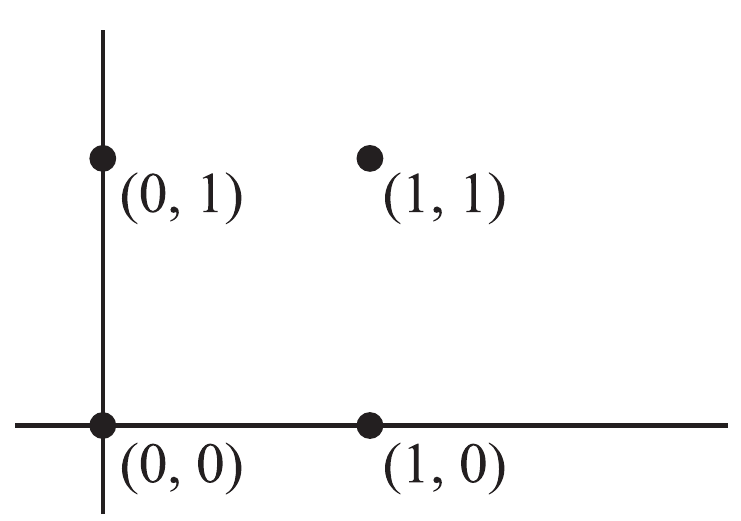
\includegraphics[width=5cm,keepaspectratio=true]{./pe/pands0101.png}
	% pands0101.png: 0x0 pixel, 300dpi, 0.00x0.00 cm, bb=
	\label{fig:0101}
\end{figure}


{Tipos de espacio muestral}
\begin{itemize}
	\item \emph{Finito:} tiene un número finito de puntos.
	\item \emph{Infinito numerable:} Tiene tantos puntos como los números naturales $\N$ (es decir, podemos numerar el espacio).
	\item \emph{Infinito no numerable:} Tiene tantos puntos como la recta real $\R.$  Por ejemplo, el intervalo $0<x<1.$
\end{itemize}



Si el espacio muestral es finito o infinito numerable, diremos que es \emph{discreto.}  Si es infinito no numerable, diremos que es \emph{continuo.}

\subsection{Eventos}

Un \emph{evento} es un subconjunto $A$ de un espacio muestral $S,$ es decir, un subconjunto de todos los posibles resultados de un experimento. Si el resultado es un elemento de $A,$ diremos que \emph{$A$ ha ocurrido.} 

Un evento que consiste de un único punto de $S$ es llamado a veces \emph{evento elemental o simple.}


\begin{figure}
	\centering
	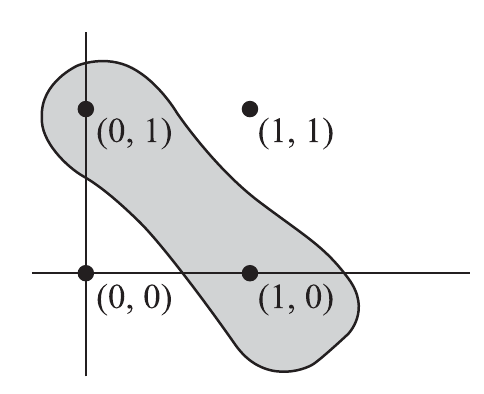
\includegraphics[height=3cm,keepaspectratio=true]{./pe/pands0102.png}
	% pands0102.png: 0x0 pixel, 300dpi, 0.00x0.00 cm, bb=
	\caption{Espacio muestral para el lanzamiento de una moneda dos veces seguidas.}
	\label{pands0102}
\end{figure}



\begin{ejemplo}
	\label{exmp:1.8}
	Si lanzamos una moneda dos veces, el evento de que obtengamos \emph{exactamente} un reverso  es un subconjunto del espacio muestral mostrado en la figura \ref{pands0102}.
\end{ejemplo}



Como eventos particulares, podemos considerar todo el espacio muestral $S$ como el \emph{evento cierto o seguro} y el conjunto vacío $\emptyset$ como el \emph{evento imposible.}


\subsection{Operaciones entre eventos} 
Supongamos que $A,B \subset S$ son dos eventos. 
\begin{itemize}
	\item $A\cup B$ es el evento \texttt{``ocurre $A$ o $B$ o ambos'',} y también es llamado \emph{unión de $A$ con $B$.}  
	\item $A\cap B$ es el evento \texttt{``ocurre $A$ y $B$'',} y también es llamado \emph{intersección de $A$ con $B$.}  
	\item $A'$ es el evento \texttt{``no ocurre $A$'',} y también es llamado \emph{negación de $A$.} 
	\item $A-B=A\cap B'$ es el evento \texttt{``ocurre $A$ pero no $B$'',} y también es llamado \emph{diferencia de $A$ menos $B.$}  Observe que
	$A' = S - A.$
\end{itemize}


Si $A\cap B= \emptyset,$ entonces diremos que \emph{$A$ y $B$} son \emph{disjuntos} o \emph{mutuamente excluyentes.} 

\begin{definicion}
	Si $A_{1},A_{2},... \subset S$ es una colección de eventos tales que $A_{i}\cap A_{j}=\emptyset$ siempre que $i\neq j,$ entonces diremos que son \emph{eventos mutuamente excluyentes}
\end{definicion}

\begin{definicion}
	Si $A_{1}, A_{2}, ...\subset S$ son eventos mutuamente excluyentes diremos que $A_{1} \cup A_{2} \cup ... $ es la \emph{unión disjunta} de tales eventos y en ese caso escribiremos
	\begin{align}
		A_{1}\sqcup A_{2} \sqcup ...
	\end{align}
\end{definicion}


\begin{definicion}
	Si \begin{align}
		S=A_{1}\sqcup A_{2} \sqcup ...
	\end{align}
	diremos que $A_{1},A_{2},...\subset S$  es una \emph{partición de $S.$}
\end{definicion}


\begin{ejemplo}
	\label{exmp:1.9}
	Respecto al experimentos de lanzar una moneda dos veces, consideremos el evento $A$ que consiste en \emph{obtener al menos un sol,}  mientras que el evento $B$ consiste en que \emph{el segundo lanzamiento sea un reverso.}
	
	Entonces $A=\set{TH,HT,HH},$ $B=\set{HT,TT}$ y por tanto 
	\begin{enumerate}
		\item $A\cup B =$ $\set{HT,TH,HH,TT}= S$ 
		\item $A\cap B =$ $\set{HT}$ 
		\item $A'=$$\set{TT}$
		\item $A-B=$$\set{TH,HH}$
	\end{enumerate}
	
\end{ejemplo}


\subsection{Enfoques de la probabilidad}

A cualquier evento en un espacio muestral se le puede asignar un número entre $0=0\%$ y $1=100\%$ que representa su \emph{probabilidad} de ocurrir.


Si un evento puede ocurrir en $h$ diferentes maneras de un total de $n$ posibles resultados, todos igualmente plausibles, entonces la probabilidad del evento es $h/n.$


\begin{ejemplo}
	\label{exmp:1.10}
	Supongamos que queremos conocer la probabilidad de que un sol aparezca en un solo volado.  Desde que hay dos maneras diferentes \emph{igualmente probables} en que la moneda caiga,  y de esas dos maneras un sol sólo puede hacerlo de una manera, razonamos que su probabilidad es $1/2.$
	
	
	\begin{observacion}
		Aquí suponemos que la moneda no está cargada.
	\end{observacion}
	
\end{ejemplo}


Si después de $n$ repeticiones de un experimento, donde $n$ es suficientemente grande, se observa que un evento ocurre en $h$ ocasiones, entonces diremos que la probabilidad del evento es $h/n.$  Esta es también llamada \emph{probabilidad empírica} del evento.


\begin{ejemplo}
	\label{exmp:1.11}
	Si lanzamos una moneda $1000$ veces y obtenemos sol 532 veces, estimamos que la probabilidad resultantes es $532/1000=0.532$.
\end{ejemplo}



\begin{observacion}
	Ambos enfoque tienen sus inconvenientes:
	\begin{enumerate}
		\item En el caso clásico, la expresión \emph{``igualmente probable''} es vaga; 
		\item mientras que en el enfoque frecuencial, \emph{``un número muy grande''} no es preciso. 
	\end{enumerate}
	Por estas razones, los matemáticos han desarrollado un \emph{enfoque axiomático} de la probabilidad.
\end{observacion}


\subsection{Los Axiomas de la probabilidad}

Supongamos que tenemos un espacio muestral $S.$ Supongamos que $C$ es la colección de todos los eventos en $S.$ Diremos que $P:C \to \R$ es una función de probabilidad si satisface las siguientes propiedades:

\begin{axioma}
	Para cada evento $A,$ se tiene que
	\begin{align}
		\label{1.1}
		P(A)\geq 0.
	\end{align}
	
\end{axioma}



\begin{axioma}
	La probabilidad del evento cierto $S$ es
	\begin{align}
		\label{1.2}
		P(S)=1.
	\end{align}
\end{axioma}



\begin{axioma}
	Para cualquier cantidad numerable de eventos mutuamente excluyentes
	$A_{1},A_{2},...$ tenemos que
	\begin{align}
		\label{1.3}
		P(A_{1}\sqcup A_{2} \sqcup ...)=P(A_{1})+P(A_{2})+...
	\end{align}
	En particular, para dos eventos mutuamente excluyentes $A_{1},A_{2},$
	\begin{align}
		\label{1.4}
		P(A_{1}\sqcup A_{2})=P(A_{1})+P(A_{2})
	\end{align}
	
\end{axioma}


\subsection{Algunos teoremas importantes en probabilidad}

\begin{teorema}
	\label{thm:1.1}
	Si $A_{1}\subset A_{2},$ entonces $P(A_{1})\leq P(A_{2})$ y
	\begin{align}
		P(A_{2}-A_{1})=P(A_{2})-P(A_{1}).
	\end{align}
\end{teorema}


\begin{teorema}
	\label{thm:1.2}
	Para cada evento $A$,
	\begin{align}
		\label{1.5}
		0\leq P(A) \leq 1,
	\end{align}
	
	es decir, la probabilidad siempre se encuentra entre $0\%$ y $100\%.$
\end{teorema}


\begin{teorema}
	\label{thm:1.3}
	El evento imposible tiene probabilidad cero, es decir,
	\begin{align}
		P(\emptyset)=0.
	\end{align}
\end{teorema}


\begin{teorema}
	\label{thm:1.4} La probabilidad de un evento complementarios está dada por
	\begin{align}
		\label{1.7}
		P(A')=1-P(A)
	\end{align}
\end{teorema}


\begin{teorema}
	\label{thm:1.5} Si $A=A_{1}\sqcup...\sqcup A_{N}$ es la unión disjunta de eventos mutuamente excluyentes entonces
	\begin{align}
		\label{1.8}
		P(A)=P(A_{1})+...+P(A_{N}).
	\end{align}
	
	
	En particular, si $S=A_{1}\sqcup...\sqcup A_{N}$ entonces
	\begin{align}
		\label{1.9}
		P(A_{1})+...+P(A_{N})=1.
	\end{align}
\end{teorema}


\begin{teorema}
	\label{thm:1.6}
	Si $A,B,C$ son dos eventos no necesariamente excluyentes, entonces
	\begin{align}
		\label{1.10}
		P(A\cup B)=P(A)+P(B)-P(A\cap B).
	\end{align}
	\begin{align}
		\label{1.11}
		P(A\cup B \cup C)&=P(A)+P(B)+P(C)\\
		&-P(A\cap B)-P(B\cap C)-P(C\cap A)\\
		&+P(A\cup B \cup C).
	\end{align}
\end{teorema}



\begin{teorema}
	\label{thm:1.7}
	Para cualesquiera eventos $A,B,$
	\begin{align}
		\label{1.12}
		P(A)=P(A\cap B)+P(A\cap B').
	\end{align}
\end{teorema}


\begin{teorema}
	\label{thm:1.8}
	Si $A_{1},A_{2},..., A_{N}$ es una partición del espacio muestral $S,$ es decir,
	$S=A_{1} \sqcup A_{2} \sqcup ... \sqcup A_{N}$ entonces para cualquier evento $A$
	\begin{align}
		\label{1.13}
		P(A)=P(A\cap A_{1})+ P(A\cap A_{2}) + ... +P(A\cap A_{N}).
	\end{align}
\end{teorema}


\subsection{Asignación de probabilidades}

Si un espacio muestral consiste en una cantidad \emph{finita} de posibles resultados $a_{1},...,a_{N},$ entonces por el teorema \ref{thm:1.5},
\begin{align}
	\label{1.14}
	P(A_{1})+...+P(A_{n})=1
\end{align}
donde $A_{1},...,A_{n}$ son \emph{conjuntos elementales} o \emph{eventos simples} dados por $A_{i}=\set{a_{i}}.$


Se sigue que uno puede escoger de manera arbitraria cualesquiera números no negativos como probabilidades de estos eventos simples, siempre que se satisfaga \eqref{1.14}. 

En particular, si suponemos \emph{probabilidades iguales} para todos los eventos, entonces
\begin{align}
	\label{1.15}
	P(A_{k})=\dfrac{1}{n}, \; k=1,2,...,n,
\end{align}
y si $A$ es un evento formado por la unión disjunta de $h$ eventos simples, entonces
\begin{align}
	\label{1.16}
	P(A)=\dfrac{h}{n}.
\end{align}


\begin{observacion}
	Esto es equivalente al \textit{enfoque clásico.} Pero podemos usar el \textit{enfoque frecuencial} para asignar dichas probabilidades.
\end{observacion}


\begin{ejemplo}
	\label{exmp:1.12}
	Si solo dado se lanza, la probabilidad de que obtengamos un 2 o un 5 es 
	\begin{equation} P(\set{2,5}) = P(\set{2}) + P(\{5\}) = 1/6 + 1/6 = 1/3. \end{equation}
\end{ejemplo}
